\chapter{Bi-Objective Optimization and Pareto Optimality\label{chap:biobjective-optimization}}

% Signposting
This chapter describes bi-objective optimization, starting with a definition of the problem and the more general case of multi-objective optimization.
We also define the notation for bi-objective optimization in the context of SAT that is used in this work.
In a second and last section, we discuss different approaches to solving bi-objective optimization problems.

\section{Multi-Objective Optimization Under Pareto Optimality\label{sec:multiopt}}

% Multiobjective optimization
Multi-objective optimization is the problem of optimizing $\nobj$ objective functions with the decision variable $x$, while $x$ is from a feasible set $\feasible$~\autocite{Ehrgott2005-1}.
W.l.o.g., we assume that all optimizations seek to minimize the objective function.
Formally a multi-objective optimization problem (MOOP) is the following:
\begin{equation}\label{eq:moop}
  \min (\generalobj_1(x),\dots,\generalobj_\nobj(x))\ \text{s.t.}\ x\in \feasible.
\end{equation}

% Pareto optimality
For multi-objective optimization problems, since the objectives might be in conflict with each other, no single optimal solution exists.
However, the notions of domination and pareto optimality can be used to define what a minimal point for multiple objective functions is.
\begin{definition}[Domination~\autocite{Ehrgott2005-2}]
  Given a MOOP as defined in \cref{eq:moop} and two solutions $x,x' \in \feasible$, $x$ dominates $x'$ (w.r.t.\ $\generalobj_1,\dots,\generalobj_\nobj$) if (i)~$\generalobj_i(x) \leq \generalobj_i(x')$ for $i=1,\dots,\nobj$, and (ii)~$\generalobj_i(x) < \generalobj_i(x')$ for some $i\in\{1,\dots,\nobj\}$.
  We represent $x$ dominating $x'$ as $x \prec x'$.
\end{definition}
\begin{definition}[Pareto optimality~\autocite{Ehrgott2005-2}]
  Given a MOOP as defined in \cref{eq:moop}, a solution $x \in \feasible$ is pareto-optimal (w.r.t.\ $\generalobj_1,\dots,\generalobj_\nobj$) iff there is no $x' \in \feasible$ such that $x' \prec x$, i.e., $x$ is not dominated by any other solution.
\end{definition}
When the objectives are clear from context, we will simply say that a solution $x$ is pareto-optimal.
Note that there can be multiple pareto-optimal solutions to a MOOP.
The set of all pareto-optimal solutions is called the pareto front (w.r.t.\ $\generalobj_1,\dots,\generalobj_\nobj$);
the tuple $(\generalobj_1(x),\dots,\generalobj_\nobj(x))$ for a pareto-optimal $x$---i.e., the image of $x$ in objective space---is a pareto point (which multiple solutions can correspond to).

\section{Bi-Objective Optimization in a SAT Context\label{sec:biopt}}

% Bi-objective optimization in a SAT context
The subset of all multi-objective optimization problems which this work provides a solving algorithm for, is \emph{bi}-objective optimization, where the number of objective functions $\nobj=2$.
Furthermore, we restrict the objective functions to be linear.
Bi-objective optimization problems can be solved by many approaches, but in this work we focus on SAT-based approaches.
We therefore formalize the problem in a context of propositional satisfiability.
An objective $\Obj$ is a multiset of literals, which allows for representing objective functions with non-unit coefficients.
The value $\Obj(\sol)$ of a truth assignment $\sol$ under $\Obj$ is $\Obj(\sol) = \sum_{l \in \Obj} \sol(l)$, i.e., the number of the literals in $\Obj$ that $\sol$ assigns to $1$. 
Weighted objectives are represented by adding a literal multiple times.
Formalizing the objectives this way and encoding the feasible set $\feasible$ as a propositional formula $\formula$ is similar to MaxSAT, where $\formula$ resembles the hard clauses while the two objectives resemble two sets of (unit) soft clauses.
With our algorithm, we consider the task of computing a representative solution for each pareto point as well as the task of enumerating all solutions in the pareto front.

% Example: A bi-objective problem
\begin{figure}
  \begin{minipage}{0.36\textwidth}
    \footnotesize
    \begin{align*}
      \formula = &\{ \texttt{As-CNF}\left(\sum_ {x \in \Obj_\inc \cup \Obj_\dec} x \geq 3 \right), \\
        &(i_1 \lor i_2),  (i_2 \lor i_3), \\
        &(d_1 \lor d_2), (d_2 \lor d_3) \} \\ \\
      \Obj_\dec =&\{ d_1,d_2, d_3\}   \\ 
      \Obj_\inc =&\{ i_1,i_2, i_3\}  
    \end{align*}
  \end{minipage}
  \;
  \begin{minipage}{0.6\textwidth}
    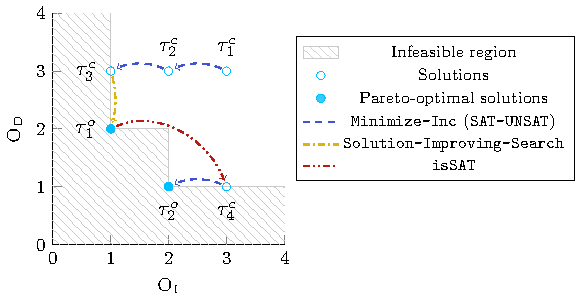
\includegraphics{search-trace.pdf}
  \end{minipage}
  \caption{Left: An example formula $\formula$ and two objectives $\Obj_\inc$ and $\Obj_\dec$.
    Right: the solution space of $\formula$ w.r.t.\ $\Obj_\inc$ and $\Obj_\dec$.
    The solutions $\tau^o_1$ and $\tau^o_2$ (solid points) are pareto-optimal, while $\tau^c_i$ for $i=1,\ldots,4$ are not.\label{fig:search-trace}}
\end{figure}
\begin{example}\label{ex:main}
  An example formula $\formula$ and two objectives $\Obj_\inc$ and $\Obj_\dec$ are shown on the left side of \cref{fig:search-trace}. 
  The solution space is illustrated on the right.
  The two solid dots correspond to the two pareto points of $\formula$ w.r.t.\ $\Obj_\inc$ and $\Obj_\dec$. 
  Examples of pareto-optimal solutions corresponding to these points are $\sol^o_1 = \{d_1, d_3, i_2, \lnot d_2, \lnot i_1, \lnot i_3\}$ and $\sol^o_2 = \{i_1, i_3, d_2, \lnot i_2, \lnot d_1, \lnot d_3\}$.
  The solution $\sol^c_3 = \{d_1, d_2, d_3, i_2, \lnot i_1, \lnot i_3\}$ is dominated by $\sol^o_1$ ($\sol^o_1 \prec \sol^c_e$) because $\Obj_\inc(\sol^o_1) \leq \Obj_\inc(\sol^c_3)$ and $\Obj_\dec(\sol^o_1) < \Obj_\dec(\sol^c_3)$.
\end{example}

% Proposition: Ordered pareto front
An important property of pareto-optimal solutions to bi-objective problems is summarized by the next proposition.
\begin{proposition}[Adapted from~\autocite{DBLP:conf/aaai/HartertS14}] \label{prop:biobjective}
  Sorting the pareto-optimal solutions of $\formula$ w.r.t.\ increasing values of $\generalobj_1$ is equivalent to sorting them w.r.t.\ decreasing values of $\generalobj_2$ and vice-versa.
\end{proposition}

% Example: Ordered pareto front
\begin{example}
  Consider the formula $\formula$, the objectives $\Obj_\inc$ and $\Obj_\dec$ and the two pareto-optimal solutions $\sol^o_1$ and $\sol^o_2$ from \cref{fig:search-trace} and \cref{ex:main}.
  By the definition of pareto-optimality, lowering the value of one objective of a pareto-optimal solution has to increase the value of the other;
  we have $\Obj_\inc(\sol^o_1) = 1 < 2 = \Obj_\inc(\sol^o_2)$ and $\Obj_\dec(\sol^o_1) = 2 > 1 = \Obj_\dec(\sol^o_2)$.
\end{example}

\section{Approaches to Bi-Objective Optimization\label{sec:approaches}}

In this section, we give an overview of different approaches to solving bi-objective optimization problems.
The focus hereby lies on the first subsection, describing SAT-based approaches.
This is because the algorithm we are proposing in this work is SAT-based and therefore other SAT-based approaches are directly competing.
In the section thereafter, we survey exact approaches based on other declarative optimization paradigms, mainly constraint and mixed integer programming.
The last section gives a brief overview of methods to approximate the pareto front, rather than finding it exactly.
In addition to approaches solving bi-objective optimization under pareto optimality, we also discuss some approaches that make use of different optimality definitions.

\subsection{SAT-Based Approaches\label{sec:sat-based}}

% Signposting
We highlight three SAT-based approaches to bi-objective optimization:
enumeration of $P$-minimal solutions, Seesaw, and enumeration of pareto-minimal correction sets.

\subsubsection{$P$-minimal Solution Enumeration\label{sec:p-minimal}}

% P-minimal solution enumeration
The approach perhaps closest to ours is solving multi-objective constraint optimization problems by enumerating so-called $P$-minimal solutions~\autocite{DBLP:conf/cp/SohBTB17,DBLP:conf/ftp/KoshimuraNFH09}.
Since this approach is so close to ours, we are using it as one of the two approaches we empirically compare \algname{} to in \cref{chap:experiments}.
The $P$-minimal approach  corresponds to enumerating the solutions of $\formula^\text{W} = \formula \land \tot(\Obj_{\inc}) \land \tot(\Obj_{\dec})$ that are subset-minimal w.r.t.\ the set of outputs of the totalizers.
More precisely, if $P$ is the set of output literals of $\tot(\Obj_{\inc}) \land \tot(\Obj_{\dec})$, then the goal is to enumerate solutions $\sol$ such that no other solution $\sol$ has $\{ l \mid l \in P \land \sol(l) = 0\} \subsetneq \{ l \mid l \in P \land \sol(l) = 0\}$.
The procedure for enumerating such solutions (detailed in~\textcite{DBLP:conf/ftp/KoshimuraNFH09}) works by (i)~using a solver to obtain any solution $\sol$ of $\formula^\text{W}$, (ii)~iteratively minimizing the subset of variables of $P$ set to true by the solution, and, once a minimal solution $\sol_m$ has been found, (iii)~adding the clause $(\ov{\Obj_{\inc}}{k_1} \lor \ov{\Obj_{\dec}}{k_2})$ containing the output variables corresponding to the lowest index set to true by $\sol_m$.

% Example: P-minimal
\begin{example}\label{ex:pmin}
  Consider the formula $\formula$ and two objectives $\Obj_\inc$ and $\Obj_\dec$ from \cref{fig:search-trace}.
  $P$-minimal starts by building two totalizers $\tot(\Obj_\inc)$ and $\tot(\Obj_\dec)$ and invoking the SAT solver on $\formula^\text{W} = \formula \land \tot(\Obj_\inc) \land \tot(\Obj_\dec)$.
  The result is satisfiable, assume the first solution obtained is $\sol^c_1 = \{i_1, i_2, i_3, d_1, d_2, d_3\}$. 
  In order to minimize $\sol^c_1$, the clause $(\ov{\Obj_\inc}{3} \lor \ov{\Obj_\dec}{3})$ is added to the SAT solver, and the solver is invoked again under the assumptions $\{ \ove{\Obj_\inc}{3}, \ove{\Obj_\dec}{3} \}$.
  The added clause blocks $\sol^c_1$ and all solutions dominated by $\sol^c_1$ from the search space.
  Assume the next solution obtained is $\sol^c_5 = \{d_1, d_3, i_1, i_3, \lnot d_2, \lnot i_2\}$. 
  Again, a clause $(\ov{\Obj_\inc}{2} \lor \ov{\Obj_\dec}{2})$ is added, and the SAT solver is queried with assumptions $\{ \ove{\Obj_\inc}{2}, \ove{\Obj_\dec}{2} \}$.
  The result is SAT, assume the solution obtained is $\sol^o_2 = \{ i_1, i_3, d_2, \lnot i_2, \lnot d_2, \lnot d_3\}$. 
  $P$-minimal then adds the clause $(\ov{\Obj_\inc}{2} \lor \ov{\Obj_\dec}{1})$ and invokes the solver again under the assumptions $\{ \ove{\Obj_\inc}{2}, \ove{\Obj_\dec}{1} \}$.
  The result is UNSAT which proves that $\sol^o_2$ is pareto-optimal. 
  To find a next pareto-optimal solution, the solver is queried without any assumptions for a new solution to start the minimization process from.
\end{example}

% P-minimal not ordered
Note that $P$-minimal has no guarantee on the order that the solutions are enumerated in. 
Intuitively, when an intermediate solution $\sol$ is found, the following SAT solver call either provides another solution that dominates $\sol$, or proves that $\sol$ is pareto-optimal.  

% Extending P-minimal to enumerate the full pareto front
As presented in~\cite{DBLP:conf/cp/SohBTB17}, the $P$-minimal approach will only enumerate a single solution per pareto point.
In our implementation we extended $P$-minimal to the task of enumerating all solutions on the pareto front.
Specifically, we add a new relaxation variable $r$ to the clause added each iteration for use as an assumption to enumerate all solutions at that pareto point:
the next SAT solver query is done including the assumption $\lnot r$, if a dominating solution is found, the clause is hardened by adding $\lnot r$ as a unit clause.
If no dominating solution is found, all solutions corresponding to the just discovered pareto point can be enumerated when removing the assumption $\lnot r$ by blocking every found solution and querying the solver again until it returns UNSAT.
If the next solution found dominates the previous one, we harden the clause added at the previous iteration by adding $\lnot r$ as a unit clause.
Once all solutions for that pareto point are enumerated, the clause is hardened.

% Example: P-minimal for full pareto front
\begin{example}
  Consider the same invocation of $P$-minimal as in \cref{ex:pmin}.
  In order to enumerate all solutions in the pareto front, the clause added in the first iteration is $(\ov{\Obj_\inc}{3} \lor \ov{\Obj_\dec}{3} \lor r_1)$ and the solver is queried again with the assumptions $\{ \ove{\Obj_\inc}{3}, \ove{\Obj_\dec}{3}, \lnot r_1 \}$.
  Since the solver will return a dominating solution, the clause added is hardened by adding the unit clause $\lnot r$ to the solver.
  The second iteration is modified similarly as the first, adding the relaxation variable $r_2$.
  In the third iteration, the added clause is $(\ov{\Obj_\inc}{2} \lor \ov{\Obj_\dec}{1} \lor r_3)$ and the solver call with assumptions $\{ \ove{\Obj_\inc}{2}, \ove{\Obj_\dec}{1}, \lnot r_3 \}$ is unsatisfiable.
  Now, by iteratively querying the solver with the assumptions $\{ \ove{\Obj_\inc}{2}, \ove{\Obj_\dec}{1} \}$ and blocking all found solutions, the set of solutions corresponding to the pareto point $(2,1)$ are enumerated.
\end{example}

\subsubsection{Enumeration of Pareto-Minimal Correction Sets\label{sec:pareto-mcs}}

% Pareto MSCes
In~\textcite{DBLP:conf/ijcai/Terra-NevesLM18a,DBLP:conf/aaai/Terra-NevesLM18,DBLP:conf/ijcai/Terra-NevesLM18} an approach for computing pareto-optimal solutions via so-called pareto-minimal correction sets (paretoMCSes) was proposed.
A paretoMCS (w.r.t.\ two objectives $\Obj_1$ and $\Obj_2$) consists of two sets of literals $(M_1, M_2)$ such that (i)~$M_1 \subset \Obj_1$ and $M_2 \subset \Obj_2$, and (ii)~there is a pareto-optimal solution $\sol$ that sets $\sol(l) = 1$ for all $l \in M_1 \cup M_2$ and $\sol(l) = 0$ for all other $l \in (\Obj_1 \cup \Obj_2) \setminus (M_1 \cup M_2)$.
In~\textcite{DBLP:conf/ijcai/Terra-NevesLM18a}, the computation of pareto-optimal solutions is reduced into the computation of paretoMCSes.
The task of computing paretoMCSes is accomplished by enumerating all subsets $S \subset  (\Obj_1 \cup \Obj_2)$ for which (i)~$\formula \land \bigwedge_{l \in  (\Obj_1 \cup \Obj_2) \setminus S} (\lnot l)$ is satisfiable, and (ii)~$\formula \land \bigwedge_{l \in  (\Obj_1 \cup \Obj_2) \setminus S'} (\lnot l)$ is unsatisfiable for all $S' \subsetneq S$.
Let $\mathcal{S}$ be the collection of all such sets.
The computation of $\mathcal{S}$ corresponds to MCS enumeration to which numerous algorithms have been proposed~\autocite{DBLP:conf/lpar/BendikC20,DBLP:conf/hvc/MorgadoLM12,DBLP:conf/sat/PrevitiMJM17}.
The pareto-optimal solutions are obtained by extracting the solutions satisfying $\formula \land \bigwedge_{l \in  (\Obj_{\inc} \cup \Obj_\dec) \setminus S} (\lnot l)$ for all $S \in \mathcal{S}$ and removing the dominated ones~\autocite{DBLP:conf/ijcai/Terra-NevesLM18a}.
The paretoMCS approach to multi-objective optimization is approximative in that it can only guarantee that a solution is pareto-optimal once the full set $\mathcal{S}$ has been computed.
Since paretoMCS enumeration is approximative in this sense, we are not comparing the performance of \algname{} to this approach, since our algorithm has the algorithmic advantage that all found solutions are immediately known to be pareto-optimal.
% In contrast, every minimal solution found during the $P$-minimal approach of~\textcite{DBLP:conf/cp/SohBTB17} and every solution returned by the $\E$ subroutine of \cref{alg:base-algorithm} is immediately known to be pareto-optimal.

% Example: A MCS that is not pareto-optimal
\begin{example}\label{ex:MCS}
  Consider the formula $\formula$ and two objectives $\Obj_\inc$ and $\Obj_\dec$ from \cref{fig:search-trace}.
  The paretoMCS enumeration procedure will return the solution $\sol = \{d_1, d_3, i_1, i_3, \lnot d_2, \lnot i_2\}$ since no solution $\sol_s$ of $\formula$ has $\{x \in \Obj_\inc \cup \Obj_\dec \mid  \sol_s(x) = 1\} \subsetneq \{d_1, d_3, i_1, i_3\}$.
  The solution $\sol$ is not pareto-optimal, but only filtered out when a solution that dominates it is enumerated.
  However, there are no guarantees on when such a dominating solution is found. 
\end{example}

\subsubsection{Implicit Hitting Set Approach: Seesaw\label{sec:seesaw}}

% Implicit hitting set approach
Implicit hitting set approaches for solving combinatorial optimization problems were first proposed in \textcite{DBLP:journals/ior/Moreno-CentenoK13}.
The overarching idea is that an optimization problem is modelled as a set $\cores$ of so-called \emph{cores} which represent an undesirable or conflicting substructure of the problem.
(Note that these cores are not necessarily equal to a core in SAT solving as described in \cref{sec:inc-sat}.)
All cores in $\cores$ need to be resolved by selecting a smallest hitting set $\hs$ that contains at least one element from each core.
However, the set $\cores$ is not explicitly know;
instead, it is defined implicitly through a separation oracle that can be used to test if a given hitting set $\hs$ intersects with all cores.
If the hitting set does not intersect with all cores, the oracle returns a core that is not hit.

% MaxHS and Seesaw
In~\textcite{DBLP:conf/cp/DaviesB13,DBLP:conf/sat/DaviesB13,DBLP:conf/cp/DaviesB11,DBLP:conf/sat/BergBP20}, an implicit hitting set algorithm for solving MaxSAT was proposed and refined;
other successful applications can be found in~\textcite{DBLP:conf/cp/IgnatievPLM15,DBLP:conf/kr/SaikkoWJ16,DBLP:conf/cade/FazekasBB18,DBLP:conf/kr/SaikkoDAJ18}.
Recently, Seesaw~\autocite{DBLP:conf/cp/JanotaMSM21} was proposed as a generalized implicit hitting set framework for bi-objective optimization.
In contrast to our work, a main ingredient in Seesaw is the idea of treating one of the objectives as a black box.
This allows for---but also requires---problem-specific instantiations of the black box.

% Seesaw in a SAT context
While the original paper presents Seesaw in general terms, in our context the Seesaw algorithm computes pareto-optimal solutions of a formula $\formula$ by maintaining a collection $\cores$ of subsets of $\Obj_\inc$ that are called \emph{cores}.
Informally speaking, every solution $\sol$ that improves on $\Obj_\dec$ needs to assign at least one literal from each core to $1$.
The algorithm works iteratively by computing a hitting set $\hs \subset \Obj_\inc$ (using an integer programming solver), i.e., a subset-minimal set of literals of $\Obj_\inc$ that intersects with each core in $\cores$, and then a solution $\sol$ that sets $\sol(o) = 1$ for each $o \in \hs$ and $\sol(o) = 0$ for each $o \in \Obj_\inc \setminus \hs$ and for which $\Obj_\dec(\sol)$ is the smallest possible value for all such solutions if one exists.
The iteration then extracts a new core that $\hs$ does not intersect with.
The pareto-optimal solutions of $\formula$ are identified by the size of the hitting set increasing.
More precisely, if the hitting set is found to increase from size $|\hs|$ to size $|\hs_2|$ with $|\hs_2|>|\hs|$, the solution $\sol$ found with a hitting set of size $|\hs|$ that has the smallest minimal value $\Obj_\dec(\sol)$ is pareto-optimal~\autocite{DBLP:conf/cp/JanotaMSM21}.

% Example: Seesaw
\begin{example}
  Consider the formula $\formula$ and two objectives $\Obj_\inc$ and $\Obj_\dec$ from \cref{fig:search-trace}. 
  Initially there are no cores, so $\cores = \emptyset$ and $\hs = \emptyset$.
  Since there is no $\sol$ that sets $\sol(u) = 0$ for each $u \in \Obj_\inc$, the iteration ends by extracting the core $\Obj_\inc$. 
  The intuition is, that any solution $\sol$ of $\formula$ sets at least one variable in $\Obj_\inc$ to $1$.
  In the next iteration, a hitting set over $\cores = \{ \Obj_\inc \}$ is computed.
  There are a number of alternatives;
  assume $\hs = \{ i_1 \}$.
  Since there is no $\sol$ that set $\sol(i_2) = \sol(i_3) = 0$, the iteration ends with extracting the core $\{ i_2, i_3\}$.
  The same intuition as earlier holds for this core.
  Assume the next hitting set computed is $\hs = \{i_2\}$.
  Now there is a $\sol$ that set $\sol(i_1) = \sol(i_3) = 0$;
  one that minimizes $\Obj_\dec(\sol)$ is $\sol^o_1 = \{d_1, d_3, i_2, \lnot d_2, \lnot i_1, \lnot i_3 \}$.
  The iteration ends with extracting the core $\core = \{i_1, i_3\}$.
  Now the intuition is that, since $\sol^o_1$ minimizes $\Obj_\dec$ over solutions that assign $\sol(u) = 0$ for every $u \notin \hs$, every solution that obtains a lower value of $\Obj_\dec$ assigns at least one literal of $\core$ to $1$ as well. 
  Now we have $\cores = \{ \Obj_\inc, \{i_2, i_3\}, \{i_1, i_3\}\}$;
  the only smallest hitting set is $\hs = \{i_3\}$.
  There is no $\sol$ that sets $\sol(i_1) = \sol(i_2) = 0$ so a new core $\{i_1, i_2\}$ is extracted. 
  Next, one possible hitting set is $\hs = \{i_1, i_3\}$.
  Since the size of the hitting set grew from $1$ to $2$, the algorithm concludes that $\sol^o_1$ is pareto-optimal. 
  The algorithm continues in this manner, finding the pareto-optimal $\sol^o_2$ in the process.
  After computing the hitting set consisting of all literals in $\Obj_\inc$, the core extracted is $\emptyset$ at which point the algorithm terminates. 
\end{example}

% Refined core extraction strategy
Note that the core-extraction strategy that only computes $\Obj_\inc \setminus \hs$ as the new core detailed in the example corresponds to what is called the weakest possible strategy in~\textcite{DBLP:conf/cp/JanotaMSM21}.
Seesaw is only feasible in practice when using a stronger core-extraction strategy---like the improved version detailed in the original Seesaw paper---since Seesaw otherwise reduces to enumerating all subsets of $\Obj_\inc$ as hitting sets~\autocite{DBLP:conf/cp/JanotaMSM21}.
Also note that, in contrast to \algname{} and $P$-minimal, extending Seesaw as it is presented in~\textcite{DBLP:conf/cp/JanotaMSM21} to support the enumeration of all pareto-optimal solutions seems non-trivial.
For a non-formal intuition note that, while Seesaw is guaranteed to find at least one solution obtaining the objective values of each pareto-optimal point, the non-deterministic hitting set computation might steer the algorithm past other solutions that obtain the same values.

\subsubsection{SAT-Based Lexicographic Optimization\label{sec:lex-opt}}

% (SAT-based) lexicographic optimization
In contrast to bi-objective optimization under pareto optimality, the objectives can also be lexicographically minimized~\autocite{Ehrgott2005-1}.
For two objectives, given a feasible set $\feasible$ and two objectives $\generalobj_1$ and $\generalobj_2$, a solution $x$ dominates another solution $x^d$ in the lexicographic sense if (a)~$\generalobj_1(x) < \generalobj_1(x^d)$, or (b)~$\generalobj_1(x) = \generalobj_1(x^d)$ and $\generalobj_2(x) < \generalobj_2(x^d)$.
Informally speaking, in contrast to pareto-optimality, lexicographic optimization imposes an explicit preference over the objectives and asks to compute a solution that minimizes $\Obj_1$ using $\Obj_2$ as a tie-breaker.
There is also earlier work on SAT-based lexicographic optimization~\autocite{DBLP:journals/ors/EhrgottG00,DBLP:conf/ijcai/ArgelichLS09,DBLP:journals/amai/Marques-SilvaAGL11}. 

% Lexicographic optimization and MaxSAT
Lexicographic optimization is closely related to the so-called multi-level optimization problem.
In particular, both can be cast as a single objective weighted optimization problem and solved with a MaxSAT solver~\autocite{DBLP:conf/ijcai/ArgelichLS09,DBLP:journals/amai/Marques-SilvaAGL11}.
In fact, many modern MaxSAT solvers exploit  multilevel properties of input instances in order to improve search efficiency~\autocite{DBLP:conf/vmcai/PaxianRB21,DBLP:conf/cp/AnsoteguiBGL12}.

\subsection{Other Declarative Optimization Paradigms\label{sec:other-approaches}}

% CP-based approaches
Beyond SAT-based approaches, multi-objective optimization has been studied in other declarative optimization paradigms.
An early algorithm that can be used in constraint programming is a lexicographic method first presented in~\textcite{Wassenhove1980}.
\Textcite{DBLP:conf/ecai/Gavanelli02} proposed a branch-and-bound-based algorithm that outperforms that presented in~\textcite{Wassenhove1980}.
This filtering algorithm was improved by the pareto constraint presented in~\textcite{DBLP:conf/cp/SchausH13,DBLP:conf/aaai/HartertS14}
The resulting search algorithm is similar to paretoMCSes in that it maintains a set $\mathcal{T}$ of solutions that do not dominate each other.
When a new solution is found, any solution it dominates is removed from $\mathcal{T}$.

% MIP-based approaches
Multi-objective optimization has also been studied in the context of mixed integer programming and zero-one-programming~\autocite{Ehrgott2005-6,Rasmussen1986,DBLP:journals/eor/AlvesC07}.
There are different algorithmic approaches in this field:
based on the Simplex algorithm~\autocite{Ehrgott2005-7,DBLP:journals/mp/EvansS73}, branch-and-bound approaches~\autocite{Adelgren2021,DBLP:journals/siamjo/SantisENR20} and based on reducing it to a different mixed integer programming problem~\autocite{DBLP:journals/jota/Sun17,DBLP:journals/ol/LuMS20,Soland1979}.

% Why we don't compare to these approaches
Our focus in this work is to develop a MaxSAT-based approach for solving bi-objective optimization problems, especially suited for problems naturally represented in propositional logic.
As such, we only compare to approaches solving the same problem (presented in \cref{sec:sat-based}) in our empirical evaluation.

\subsection{Probabilistic and Meta-Heuristic Approaches\label{sec:approximative}}

% Approximative vs. exact methods
Other than the exact algorithms presented so far, there are also probabilistic and mate-heuristic search algorithms for multi-objective optimization problems~\autocite{Saini2021}.
These algorithms are \emph{not} guaranteed to return the exact pareto front, but they will return good solutions that might be sufficiently close approximations.
Probabilistic and meta-heuristic algorithms are mainly used for problems that are too large to solve them with exact methods under given research constraints.
Comparing exact with approximative approaches does not necessarily give much insight, however for the sake of completeness we are giving a short overview of these approximative methods as well.

% Simulated annealing
The first category of approximative algorithms is the family of simulated annealing algorithms~\autocite{Saini2021}.
These probabilistic and meta-heuristic algorithms model the annealing process that is used to increase the quality of crystalline structure in metals.
It was first proposed in~\textcite{DBLP:journals/science/KirkpatrickGV83} and extended to multiple objectives in~\textcite{DBLP:journals/tec/BandyopadhyaySMD08}.
An example of an algorithm building on multi-objective simulated annealing can be found in~\textcite{DBLP:journals/isci/SenguptaS18}.

% Evolutionary algorithms
A second big group of algorithms are evolutionary algorithms~\autocite{Saini2021,Dasgupta2013}.
These meta-heuristic algorithms hold a set of candidate solutions referred to as \emph{population}, which is then developed over multiple iterations to approximate the pareto front;
this process simulates evolution in nature, hence the name.
Algorithms for this category were presented for example in~\textcite{DBLP:journals/jgo/StornP97,DBLP:journals/tec/DebAPM02}.